\documentclass[12pt,a4paper]{article}
\usepackage{geometry}
\geometry{a4paper, margin=1in}

\usepackage[utf8]{inputenc}

\usepackage{hyperref}
\usepackage{url}
\usepackage{caption}

\usepackage{float}
\usepackage{amsmath}
\usepackage{graphicx}
\usepackage{booktabs}

\usepackage[backend=biber, style=authoryear, citestyle=authoryear]{biblatex}
\addbibresource{references.bib}

\usepackage{listings}
\usepackage{color}

\definecolor{codegreen}{rgb}{0,0.6,0}
\definecolor{codegray}{rgb}{0.5,0.5,0.5}
\definecolor{codepurple}{rgb}{0.58,0,0.82}
\definecolor{backcolour}{rgb}{0.99,0.99,0.99}

\lstdefinestyle{mystyle}{
    backgroundcolor=\color{backcolour},   
    commentstyle=\color{codegreen},
    keywordstyle=\color{magenta},
    numberstyle=\tiny\color{codegray},
    stringstyle=\color{codepurple},
    basicstyle=\ttfamily\footnotesize,
    breakatwhitespace=false,         
    breaklines=true,                 
    captionpos=b,                    
    keepspaces=true,                 
    numbers=left,                    
    numbersep=5pt,                  
    showspaces=false,                
    showstringspaces=false,
    showtabs=false,                  
    tabsize=2
}

\lstset{style=mystyle}

{
\title{
    
\includegraphics[width=0.4\textwidth]{/Users/nicolasxx/documents/images/tsukuba-logo.png} \\
    \textbf{Experiment Design in Computer Science, Report 1} \\
    \vspace{3mm}    
    Investigating the Efficacy of U-Net Models for Detecting Adaptive Steganography in Images
}

\author{Mamanchuk Mykola, SID.202420671}
\date{12/05/2024}
}

\begin{document}

\maketitle

\section{Introduction}

Adaptive steganography methods (ASM) pose significant challenges in the field of digital security, particularly through unsanctioned leakage of information using seemingly innocuous media like digital images. These methods involve embedding malicious data into digital images, which can facilitate unauthorized activities such as remote code execution, hidden communication, and data compromise. Given the sophistication of these methods, there is a pressing need for effective detection systems that can identify and neutralize such threats without significantly compromising the utility of the carrier media.

Traditional steganography detection systems focus on altering potential carriers to destroy hidden data. However, these systems often modify the carrier's statistical and physical properties to an extent that its usability is significantly reduced. This limitation underscores the need for more sophisticated solutions that can maintain the integrity of the media while effectively identifying steganographic modifications.

Recent advances in machine learning, particularly the application of transformers and other deep learning models, have demonstrated remarkable success in complex tasks across various domains including natural language processing and image modification. These models have proven capable of decrypting complex cryptographic systems and detecting subtle anomalies in data patterns. Consequently, this study aims to explore the application of advanced machine learning model, specifically Image Segmentation models like U-Net, to determine their effectiveness in identifying and localizing bit-carriers in images that may be involved in malicious activities using ASM.

\section{Experiment Setup and Preliminary Considerations}

The objective of this experiment is to assess the efficacy of machine learning models, specifically U-Net, in detecting steganographic alterations made by advanced steganography methods. The study focuses on two sophisticated and well-documented steganography techniques, HUGO (Highly Undetectable SteGanography) and WOW (Wavelet Obtained Weights), both of which are known for their distinct and intricate embedding algorithms. These methods were chosen due to their recognition and documentation by researchers at Binghamton University, NY, USA, which also provides a comprehensive online resource [1] with C++ implementations and compiled binaries, facilitating their widespread application in experiments across various systems.

For the machine learning model, a custom U-Net architecture was selected. U-Net, originally designed for biomedical image segmentation, has been widely adopted due to its efficiency and effectiveness in various image analysis tasks. While there are advanced versions of U-Net, such as U-Net\(^2\), which offer potentially higher performance through more complex structures and additional hyperparameters, the original U-Net architecture was deemed more appropriate for this initial study. This decision was influenced by the need for a simpler, more manageable model that could be effectively tuned without the complexities associated with more sophisticated variants.

Additionally, the experiment utilizes a [2] dataset comprising 10,000 RGB images, each sized \(512 \times 512\) pixels, provided by the same research team at Binghamton University. These images serve as the foundation for training and testing the U-Net model, ensuring that the experiment is grounded in a robust dataset representative of real-world conditions where ASM might be employed.

\section{Defining Experiment, Evaluation Metrics, Tools, and Environment}

\subsection{Metrics Definition}
The effectiveness of the image segmentation model in detecting steganographic modifications will be quantitatively assessed using two primary metrics: Intersection over Union (IoU) and a simple labeling accuracy coefficient.

The IoU, also known as the Jaccard Index, is defined as:
\[
J(Y_{\text{bit}}^{\hat{}}, Y_{\text{bit}}) = \frac{|Y_{\text{bit}}^{\hat{}} \cap Y_{\text{bit}}|}{|Y_{\text{bit}}^{\hat{}} \cup Y_{\text{bit}}|}
\]
where \( Y_{\text{bit}}^{\hat{}} \) and \( Y_{\text{bit}} \) are the predicted and actual binary masks of steganographic data in the images, respectively.

Accuracy (\( A_{\text{LB}} \)) is calculated as the proportion of correctly identified pixels, defined by:

\[
A_{\text{LB}} = \frac{\sum_{i=0}^{511} \sum_{j=0}^{511} \left( \begin{array}{cc}
1 & \text{if } Y_{ij}^{\hat{}} = Y_{ij} \\
0 & \text{otherwise}
\end{array} \right)}{512^2}
\]

\subsection{Preparation of Data}
To facilitate a comprehensive analysis, 10,000 RGB images will be manipulated to generate four sets of steganographic images using the compiled binaries of the HUGO and WOW methods, each at 10\% and 25\% data filling ratios. Each original image will undergo the following process to create corresponding mask images:
\begin{enumerate}
    \item Pixel-wise subtraction between the original and the modified image.
    \item In the resulting array, non-zero values are replaced with 255, highlighting the altered pixels.
    \item Each modified image is paired with its corresponding mask to form the dataset for model training and evaluation.
\end{enumerate}
This process is repeated for each steganographic method and filling ratio to ensure that each class is represented equally in the dataset.

\subsection{Visualization of Data Preparation}

To better understand the impact of the steganographic methods and the effectiveness of the masks in highlighting modifications, visual examples of the original, stego, and corresponding mask images are provided. These examples demonstrate the subtlety of changes between the original and stego images, as well as the clear distinctions captured by the masks at different filling ratios.

\setlength{\fboxsep}{0pt} % Removes padding around the image
\setlength{\fboxrule}{0.5pt} % Sets the thickness of the border

\begin{figure}[ht]
    \centering
    \fbox{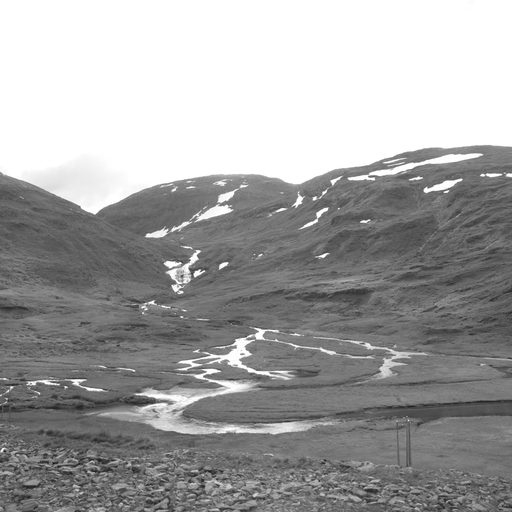
\includegraphics[width=0.32\textwidth]{images/Stego_Demo/NORMAL_1.png}}
    \fbox{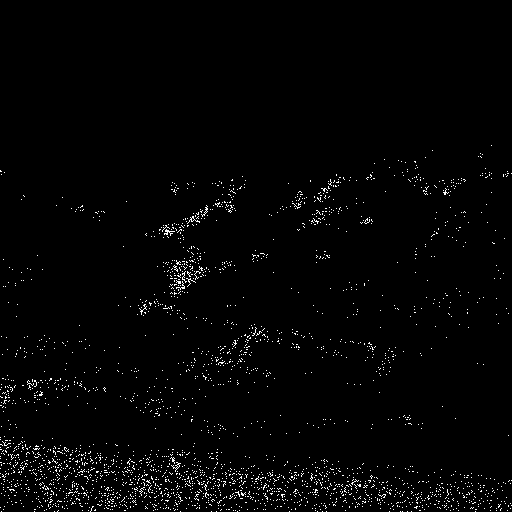
\includegraphics[width=0.32\textwidth]{images/Stego_Demo/MASK-WOW-10_1.png}}
    \fbox{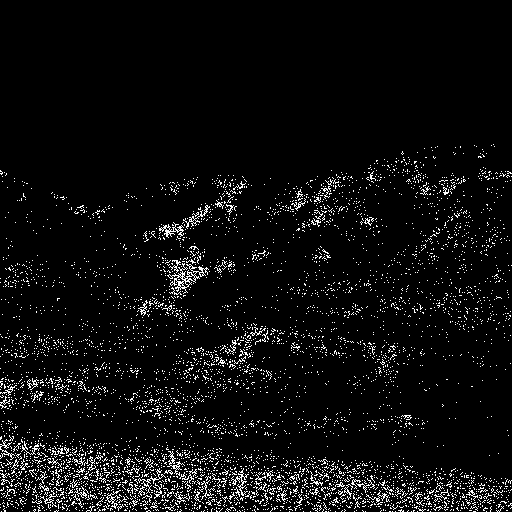
\includegraphics[width=0.32\textwidth]{images/Stego_Demo/MASK-WOW-25_1.png}}
    \caption{From left to right: Original Image, Mask for WOW 10\%, Mask for WOW 25\%.}
\end{figure}

\begin{figure}[ht]
    \centering
    \fbox{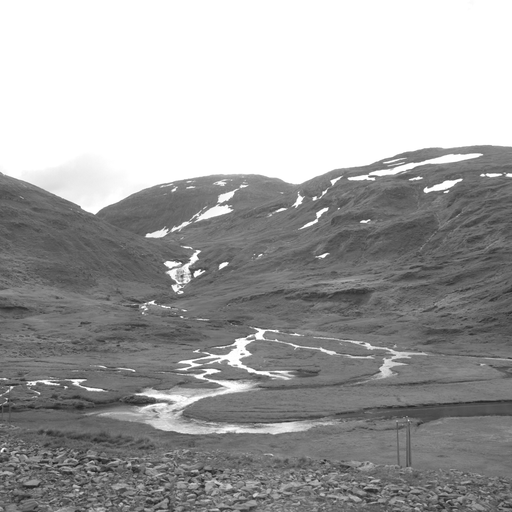
\includegraphics[width=0.32\textwidth]{images/Stego_Demo/STEGO-HUGO-25_1.png}}
    \fbox{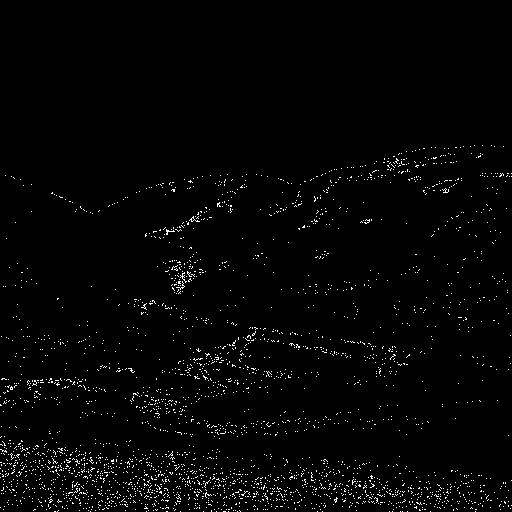
\includegraphics[width=0.32\textwidth]{images/Stego_Demo/MASK-HUGO-10_1.png}}
    \fbox{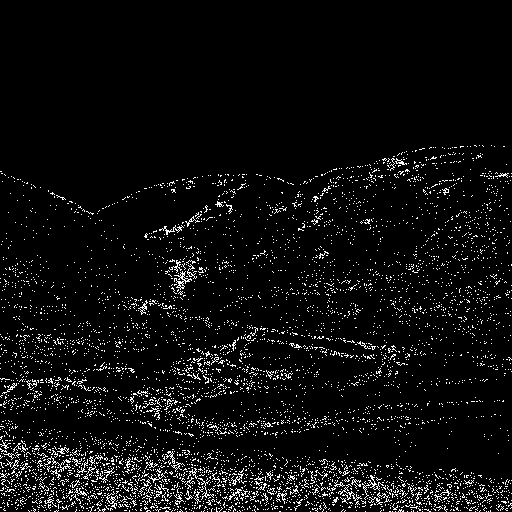
\includegraphics[width=0.32\textwidth]{images/Stego_Demo/MASK-HUGO-25_1.png}}
    \caption{From left to right: Stego Image (HUGO 25\%), Mask for HUGO 10\%, Mask for HUGO 25\%.}
\end{figure}

Each pair of stego image and its corresponding mask shows how the steganographic embedding modifies the image pixels, which are effectively highlighted by the mask. The masks reveal the regions of change, affirming the model's potential to focus on these altered areas during the detection process. The original image compared with the stego image (HUGO 25\%) visually emphasizes that there are no discernible differences to the naked eye, underscoring the challenge of detecting such modifications without sophisticated tools like the U-Net model.


\subsection{Image Sets and Experiment Design}
The prepared images are divided into specific sets for training, validation, and testing:
\begin{itemize}
    \item 8075 images for training,
    \item 950 images for validation,
    \item 475 images for ongoing testing during model epochs,
    \item 500 images for an independent final test to assess model generalization.
\end{itemize}

Additional steps include ensuring all mask images are distinctly different across the four steganographic cases and converting all images into a compatible format (.npz) for efficient processing by the model.

\subsection{Model Architecture and Training Details}

The U-Net architecture employed in this experiment is specifically designed for image segmentation tasks by [3], featuring a symmetric structure with an encoder and decoder path, which helps in capturing context and precisely locating objects in images.
 
\subsubsection{Encoder}
The encoder path consists of a series of convolutional and max pooling layers:
\begin{itemize}
    \item The first convolutional layer (Conv1) applies 64 3x3 filters to the input image, producing 64 feature channels of size 512x512.
    \item This is followed by a max pooling layer (Pool1) which reduces the spatial dimensions by half, resulting in a feature map of size 256x256x64.
    \item Subsequent convolutional layers increase the depth of feature maps while max pooling layers continue to reduce spatial dimensions. For example, the second convolutional layer (Conv2) applies 128 3x3 filters, yielding a feature map of size 256x256x128.
    \item By the fifth convolutional layer (Conv5), the spatial dimensions are reduced to 32x32, and the number of channels is increased to 1024.
    \item Each convolutional layer is followed by a dropout layer with a dropout rate of 0.5, aiding in preventing overfitting.
\end{itemize}

\subsubsection{Decoder}
The decoder path uses upsampling and concatenation to restore the spatial dimensions of the target:
\begin{itemize}
    \item The first step in the decoder (Up6) uses a 2x2 upsampling layer to double the dimensions of the input from the last encoder layer (Drop5) to 64x64.
    \item Concatenation operations (e.g., merge layer Merge6) combine feature maps from the decoder with corresponding feature maps from the encoder to retain context.
    \item The convolution layer (Conv6) then applies 512 3x3 filters, maintaining the spatial dimensions while reducing the number of feature channels to 512.
    \item This process is repeated until the final convolution layer (Conv10) restores the dimensions to 512x512, with the number of channels reduced to one, representing the pixel-by-pixel predicted map for segmentation.
\end{itemize}

For a detailed implementation of the model, see the Python code provided in Appendix A.

\subsection{Automation and Preliminary Testing}
Scripts are prepared to automate the tasks of image processing, model training, and logging. Model checkpoints are created after every epoch to monitor progress and facilitate recovery in case of interruptions. A smaller subset of the data, reduced by a factor of ten, is used initially to fine-tune hyperparameters and validate model improvements through iterative testing.

\subsection{Initiating the Experiment}
With preparations complete, the experiment is set to commence. The iterative testing and tuning phase ensures the model's efficacy before it is subjected to the full dataset, paving the way for a robust evaluation of its capabilities in detecting ASM within images.

\subsection{Environment and Hardware}

The experiment was conducted using the following robust hardware and software setup to ensure reliable and efficient processing. Let's look at the detalis of the environment:

\begin{itemize}
    \item \textbf{CPU}: Intel Xeon Silver 4110 @ 2.10GHz, 32 cores
    \item \textbf{Memory}: 64GB DDR4 DRAM
    \item \textbf{Operating System}: Linux Ubuntu 22.04 LTS
    \item \textbf{Development Environment}: PyCharm 3.12 with Python 3.8
    \item \textbf{Shell Environment}: BASH
\end{itemize}

\section{Results and Their Analysis}

\subsection{Introduction to Achieved Performance}

For the sake of keeping this paper relatively simple, I shall present only the results of the training and testing phases for the HUGO-25 model across various epochs.
For those who wish to look at various graphs and some more detailed results, I shall provide a link to a Google Drive .xlss: [4].

\subsubsection{Training Results}
\begin{tabular}{|c|c|c|c|c|}
\hline
\textbf{Epoch} & \textbf{IoU Score} & \textbf{Accuracy} & \textbf{Loss} & \textbf{Mean Absolute Error} \\
\hline
1 & 0.1902 & 93.24\% & 0.9741 & 0.0849 \\
2 & 0.3298 & 95.27\% & 0.7933 & 0.0584 \\
3 & 0.4459 & 96.62\% & 0.6587 & 0.0418 \\
\hline
\end{tabular}

\subsubsection{Independent Test Set Results}
\begin{tabular}{|c|c|c|c|c|}
\hline
\textbf{Epoch} & \textbf{IoU Score} & \textbf{Accuracy} & \textbf{Loss} & \textbf{Mean Absolute Error} \\
\hline
1 & 0.1420 & 93.35\% & 1.1014 & 0.0737 \\
2 & 0.2136 & 95.25\% & 1.0628 & 0.0511 \\
3 & 0.2645 & 95.40\% & 1.0308 & 0.0493 \\
\hline
\end{tabular}

\vspace{3mm}

Here we can notice a substantial improvement in IoU considering both training and testing sets. The IoU score rises monotonically hence an even higher result can be expected for the consequent epochs. Being limited in time, I, fortunately, leave this for those lucky to be not indifferent.

\subsection{Performance Evaluation for HUGO-25 for an individual example}

The performance metrics for the HUGO-25 model over various epochs during training and testing phases are presented below.
As we 

\subsubsection{Training and Testing Performance}
\begin{tabular}{|c|c|c|c|c|}
\hline
\textbf{Phase} & \textbf{Epoch} & \textbf{IoU} & \textbf{Accuracy} & \textbf{Set} \\
\hline
Training & 1 & 0.2695 & 88.63\% & Train \\
Testing & 1 & 0.2242 & 85.81\% & Test \\
Training & 2 & 0.4372 & 94.77\% & Train \\
Testing & 2 & 0.4175 & 94.23\% & Test \\
Training & 3 & 0.4813 & 95.38\% & Train \\
Testing & 3 & 0.4344 & 94.23\% & Test \\
\hline
\end{tabular}

\vspace{2mm}
\textit{Note: The IoU and Accuracy metrics are presented for both training and independent testing images, highlighting the model's learning progression and generalization capability across epochs.}

\vspace{2mm}

As the section's name states, here we can see evaluation results for an individual image.
Also, there is a drastic change in the IoU/Accuracy ratio, which has to do with my modifying the threshold for a single image of a pixel-wise prediction to be considered a data carrier (i.e. directly modified threshold, which typically is inaccessible in the model itself i.e. for an average result, which is a shame).
A proceeding conclusion states that the lesser the Accuracy (i.e. amount of marked pixels) the higher the IoU ratio. Up to a certain point, it is true, as once we try to mark more and more pixels, the actual amount of incorrectly marked units inevitably rises due to the used cross-entropy loss and overall randomness of confidence related to Xavier initialization of weights, etc. This is a much more promising research which I shall be, perhaps, looking forward to investigating in the second report.

\subsubsection{Visual Results for Epochs 1 and 3}

\paragraph{Epoch 1 - Training Set Image - Results for HUGO, filling ratio 25\%}
\captionsetup{skip=0pt}

{
\centering
\makebox[\textwidth]{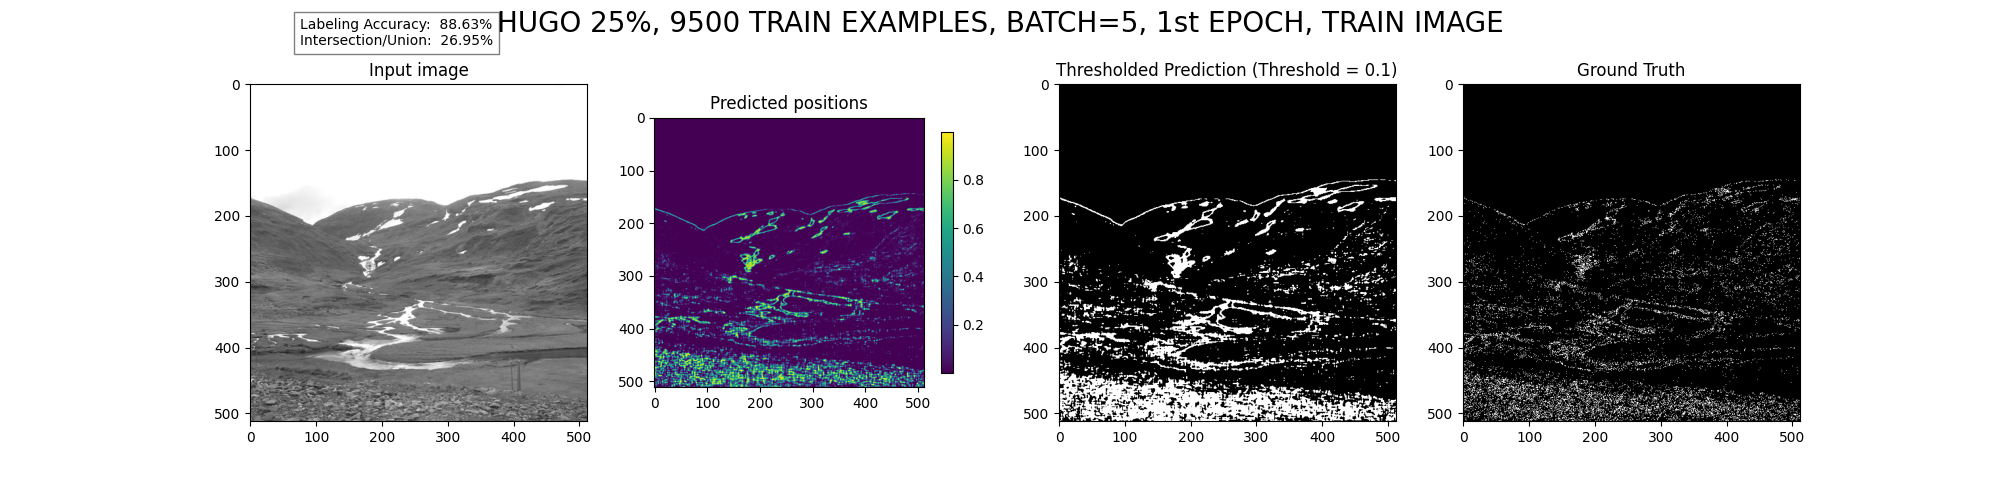
\includegraphics[width=1.3\textwidth]{images/Results/HUGO-25_-9500-TRAIN-EXAMPLES-BATCH=1-1st-EPOCH-TRAIN-IMAGE.png}}
\captionof{figure}{Training results for Epoch 1. Left to right: Input image, Predicted positions, Thresholded prediction, Ground truth. Labeling Accuracy: 85.81\%, IoU: 22.42\%.}

\paragraph{Epoch 1 - Test Set Image - Results for HUGO, filling ratio 25\%}
\makebox[\textwidth]{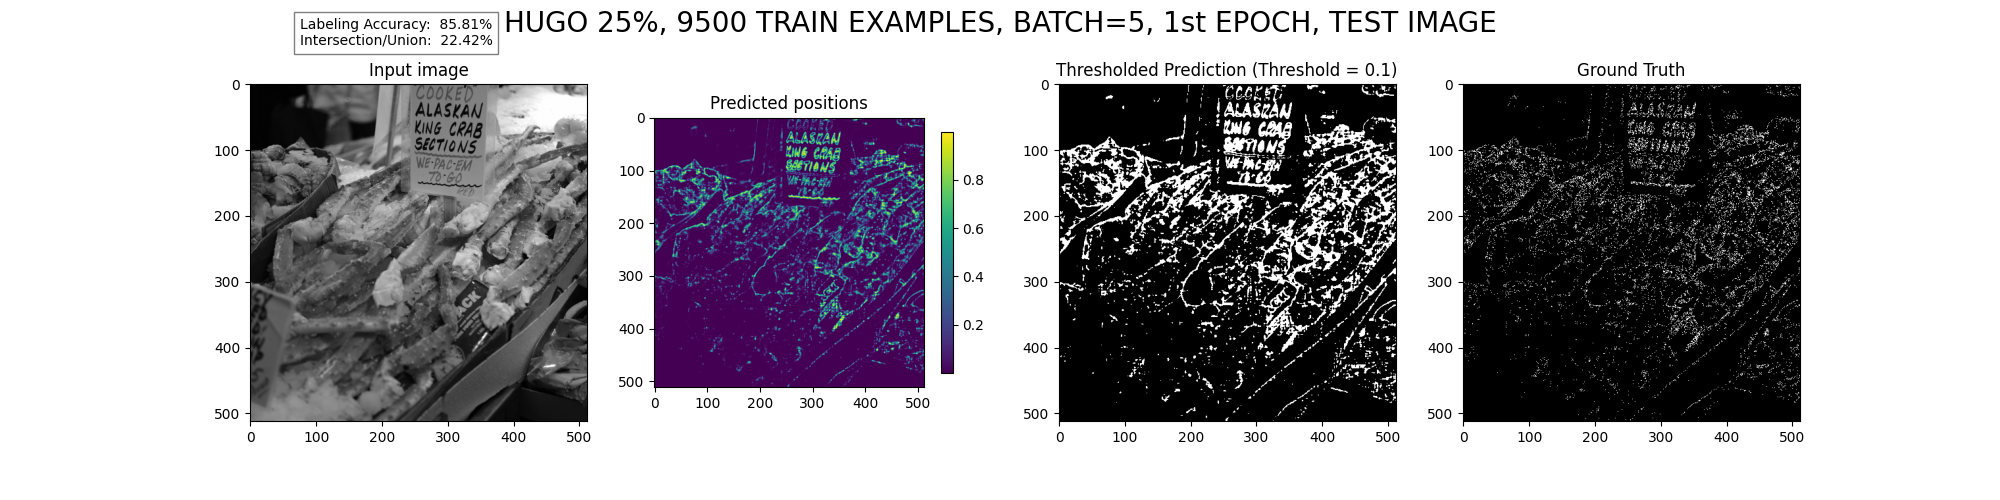
\includegraphics[width=1.3\textwidth]{images/Results/HUGO-25_-9500-TRAIN-EXAMPLES-BATCH=1-1st-EPOCH-TEST-IMAGE.png}}
\captionof{figure}{Testing results for Epoch 1. Labeling Accuracy: 85.81\%, IoU: 22.42\%.}

\paragraph{Epoch 3 - Training Set Image - Results for HUGO, filling ratio 25\%}
\makebox[\textwidth]{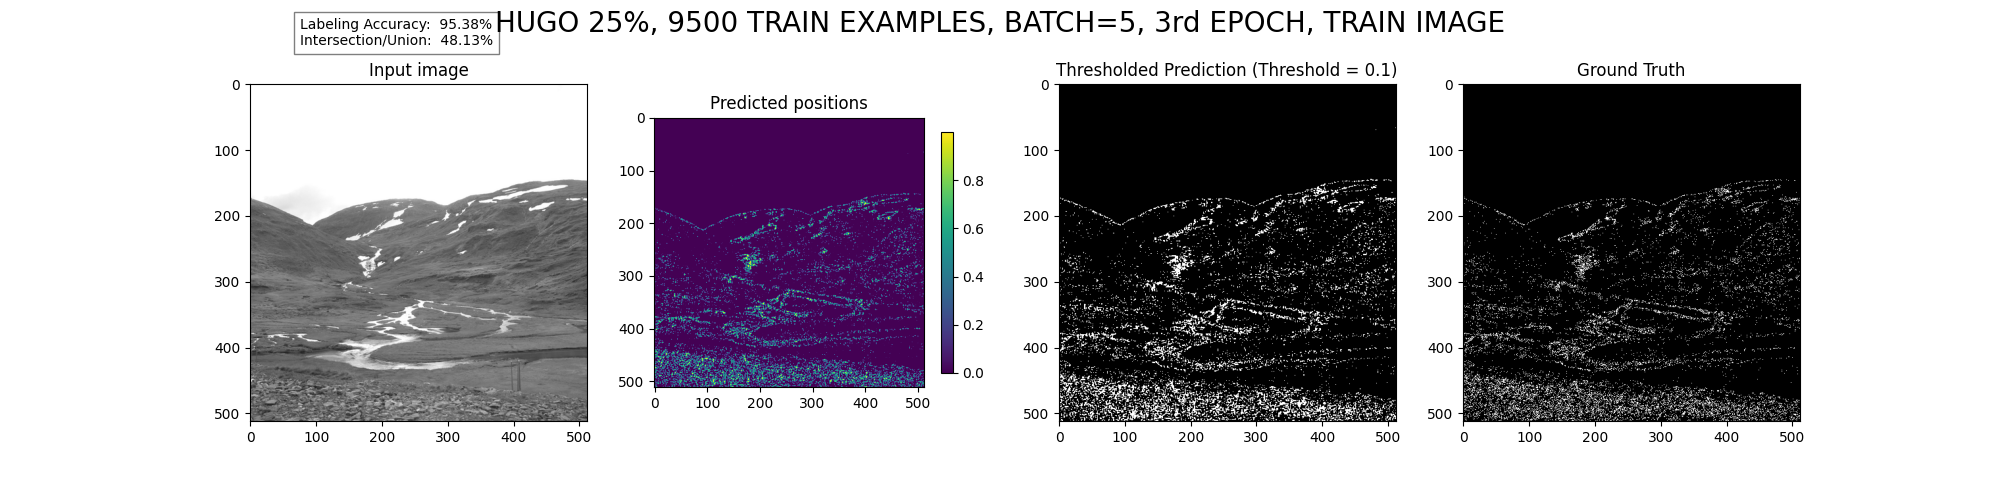
\includegraphics[width=1.3\textwidth]{images/Results/HUGO-25_-9500-TRAIN-EXAMPLES-BATCH=1-3rd-EPOCH-TRAIN-IMAGE.png}}
\captionof{figure}{Training results for Epoch 3. Labeling Accuracy: 95.38\%, IoU: 48.13\%.}

\paragraph{Epoch 3 - Test Set Image - Results for HUGO, filling ratio 25\%}
\makebox[\textwidth]{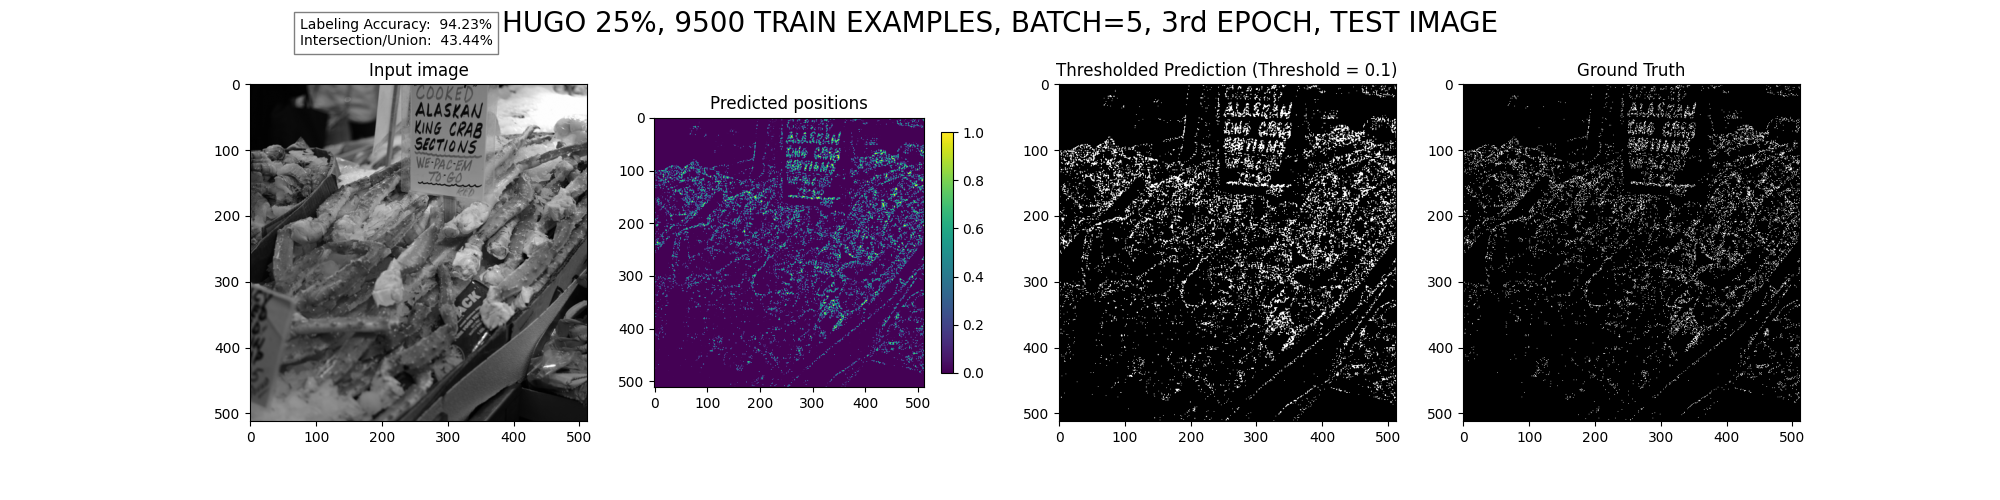
\includegraphics[width=1.3\textwidth]{images/Results/HUGO-25_-9500-TRAIN-EXAMPLES-BATCH=1-3rd-EPOCH-TEST-IMAGE.png}}
\captionof{figure}{Testing results for Epoch 3. Labeling Accuracy: 94.23\%, IoU: 43.44\%.}
}

\captionsetup{skip=10pt}

\subsection{Discussion}

The incremental improvements in both IoU and accuracy across epochs indicate effective learning by the model, with IoU showing particularly significant gains. This suggests that the model becomes better at segmenting relevant features from the background over time. However, a notable observation is the slower increase in accuracy compared to IoU, which can be attributed to the model becoming more precise in its predictions, albeit at a slower rate.

Further studies could explore adjusting the threshold for pixel classification, which, as observed, affects the IoU and accuracy differently. A higher threshold might decrease overall accuracy but can significantly enhance the IoU, suggesting a more focused prediction by the model.

\section{Estimation of Test Results}

The introduction of confidence intervals is crucial for understanding the fluctuation of results within our experiments. Despite the large volume of images analyzed, minor deviations are inherent due to factors such as cross-entropy losses and Xavier initialization during model training. There is a notable absence of human bias in data selection, given that the dataset was predetermined. However, the variability in results highlights the stochastic nature of the learning algorithms employed.

To account for the inherent variability, particularly in the IoU measurements which are more prone to fluctuation, confidence levels of 90\% and 95\% were chosen for IoU and \( A_{\text{LB}} \) metrics, respectively. These correspond to Z-scores of 1.645 for IoU and 1.96 for \( A_{\text{LB}} \).

The standard deviation is computed using the formula:
\[
\sigma = \sqrt{\frac{\sum_{i=1}^{n} (\bar{X} - X_i)^2}{n-1}}
\]
where $\bar{X}$ is the sample mean and $n$ is the number of examples.

The confidence intervals are then defined by:
\[
\Delta = \bar{X} \pm z \frac{\sigma}{\sqrt{n}}
\]

The full computation algorithm is attached in Appendix B.

\subsection{Deviation Estimate Using Confidence Intervals}

The following table summarizes the calculated mean, standard deviation, and confidence intervals for every case and each metric:

\begin{table}[h]
\centering
\begin{tabular}{@{}lllll@{}}
\toprule
Case & Mean & Std Dev & $\Delta$, .5f & Confidence Interval \\ \midrule
HUGO-10 Accuracy & 0.9802 & 0.0018 & ±0.00016 & [0.9801, 0.9804] \\
HUGO-10 IoU & 0.1974 & 0.0037 & ±0.00027 & [0.1971, 0.1977] \\
HUGO-25 Accuracy & 0.9540 & 0.0022 & ±0.00020 & [0.9538, 0.9542] \\
HUGO-25 IoU & 0.2645 & 0.0046 & ±0.00034 & [0.2642, 0.2649] \\
WOW-10 Accuracy & 0.9785 & 0.0021 & ±0.00019 & [0.9783, 0.9787] \\
WOW-10 IoU & 0.1884 & 0.0039 & ±0.00029 & [0.1881, 0.1887] \\
WOW-25 Accuracy & 0.9459 & 0.0026 & ±0.00023 & [0.9456, 0.9461] \\
WOW-25 IoU & 0.1887 & 0.0052 & ±0.00039 & [0.1883, 0.1891] \\ \bottomrule
\end{tabular}
\caption{Summary of test results with confidence intervals}
\end{table}

\subsection{Conclusion}
The following report discloses results of a new approach to steganography analysis. While many images have been analyzed using an advanced ML Model for image segmentation, our results can still be enhanced by performing more epochs on the data. Additionally, studying the coherence between a labeling threshold and IoU with Accuracy presents a promising direction for future development. Moreover, the resulting model has proven effective in potentially destructing stegoimages, which provides a solid foundation for future advancements in this perspective. The final results, specifying intervals, offer insights into the actual deviation of obtained results considering the utilized methodologies.

\section*{References}
\begin{enumerate}
    \item \textbf{Binghamton University}, Steganography Algorithms, 2021. Available online: \url{https://dde.binghamton.edu/download/stego_algorithms/} [Accessed: 2024-05-12]
    \item \textbf{Binghamton University}, BOSSbase 1.01 Image Database, 2021. Available online: \url{https://dde.binghamton.edu/download/ImageDB/BOSSbase_1.01.zip} [Accessed: 2024-05-12]
    \item \textbf{GitHub Community}, Implementation of deep learning framework -- Unet, using Keras, 2018. Available online: \url{https://github.com/zhixuhao/unet} [Accessed: 2024-05-12]
    \item \textbf{Nicolas M., your private reseracher for hire}, Graphs and detailed results of proceeding steganographic research, 2024. Available online: \url{https://docs.google.com/spreadsheets/d/1LniEilwf_e4bVGqWlbKMMRLX5dWR2YHe/edit?usp=drive_link&ouid=100727652948933857957&rtpof=true&sd=true} [Last update: 2077-12-10]
\end{enumerate}

\newpage  % or \clearpage if you have pending floats like figures or tables
\section*{Appendix A: U-Net Model Implementation}

The following Python code details the implementation of the U-Net model used in this study. This code utilizes the Keras framework with TensorFlow as the backend.

\begin{lstlisting}
from keras.layers import Input, Conv2D, MaxPooling2D, UpSampling2D, Dropout, concatenate
from keras.models import Model
from tensorflow import keras
import tensorflow as tf

def unet(pretrained_weights=None, input_size=(256, 256, 1), activation='relu'):
    inputs = Input(input_size)
    # Encoder
    conv1 = Conv2D(64, 3, activation=activation, padding='same', kernel_initializer='he_normal')(inputs)
    conv1 = Conv2D(64, 3, activation=activation, padding='same', kernel_initializer='he_normal')(conv1)
    pool1 = MaxPooling2D(pool_size=(2, 2))(conv1)
    ...
    # Decoder
    up6 = Conv2D(512, 2, activation=activation, padding='same', kernel_initializer='he_normal')(
        UpSampling2D(size=(2, 2))(drop5))
    merge6 = concatenate([drop4, up6], axis=3)
    conv6 = Conv2D(512, 3, activation=activation, padding='same', kernel_initializer='he_normal')(merge6)
    ...
    model = Model(inputs, conv10)
    model.compile(optimizer='adam', loss='binary_crossentropy', metrics=['accuracy'])
    return model
\end{lstlisting}

\newpage

\section*{Appendix B: Standard Deviation Computation}

The following Python code gives a hint on how confidence intervals are computed:

\begin{lstlisting}
    import numpy as np
    import math
    
    # Loading the results from file
    loaded_arrays = np.load('code_py/Results.npy', allow_pickle=True).item()
    
    # Calculating standard deviation
    def compute_std_dev(data):
        if len(data) < 2:
            raise ValueError("Standard deviation requires at least two data points.")
        
        mean = sum(data) / len(data)
        variance = sum((x - mean) ** 2 for x in data) / (len(data) - 1)
        std_dev = math.sqrt(variance)
        return std_dev
    
    # Defining confidence levels for each metric, i.e. 90 and 95%
    z_scores = {
        "HUGO-10-ACCURACY": 1.96,
        "HUGO-10-IOU": 1.645,
        "HUGO-25-ACCURACY": 1.96,
        "HUGO-25-IOU": 1.645,
        "WOW-10-ACCURACY": 1.96,
        "WOW-10-IOU": 1.645,
        "WOW-25-ACCURACY": 1.96,
        "WOW-25-IOU": 1.645
    }
    
    # Computing standard deviations and confidence intervals
    results = {}
    for key, data in loaded_arrays.items():
        std_dev = compute_std_dev(data)
        mean = sum(data) / len(data)
        z_score = z_scores[key]
        # Calculating the margin of error
        margin_of_error = z_score * (std_dev / math.sqrt(len(data)))
        lower_bound = mean - margin_of_error
        upper_bound = mean + margin_of_error
        results[key] = (mean, std_dev, lower_bound, upper_bound, margin_of_error)
    
    # Saving the results to a text file
    output_filename = 'Deviations_and_intervals.txt'
    with open(output_filename, 'w') as file:
        for name, (mean, std, lower, upper, margin) in results.items():
            file.write(f"{name}: Mean = {mean:.4f}, Std Dev = {std:.4f}, MoE = ~{margin:.5f}, CI = [{lower:.4f}, {upper:.4f}]\n")
    print(f"Results written to {output_filename}")
\end{lstlisting}

\end{document}